
%%%%%%%%%%%%%%%%%%%%%%%%%%%%%%%%%%%%%%%%%%%%%%%%%%%%%%%%%%%%%%%%%%%%%%%%%%%%%%%%%%%%%%%%%%%%%
% Setup title, etc in config.tex
%%%%%%%%%%%%%%%%%%%%%%%%%%%%%%%%%%%%%%%%%%%%%%%%%%%%%%%%%%%%%%%%%%%%%%%%%%%%%%%%%%%%%%%%%%%%%

%%%%%%%%%%%%%%%%%%%%%%%%%%%%%%%%%%%%%%%%%%%%%%%%%%%%%%%%%%%%%%%%%%%%%%%%%%%%%%%%%%%%%%%%%%%%%
%Page Layout
%%%%%%%%%%%%%%%%%%%%%%%%%%%%%%%%%%%%%%%%%%%%%%%%%%%%%%%%%%%%%%%%%%%%%%%%%%%%%%%%%%%%%%%%%%%%%


\def\myPageLayout{twoside}
%\def\myPageLayout{oneside}


%%%%%%%%%%%%%%%%%%%%%%%%%%%%%%%%%%%%%%%%%%%%%%%%%%%%%%%%%%%%%%%%%%%%%%%%%%%%%%%%%%%%%%%%%%%%%
% Personal data and user ad-hoc commands
%%%%%%%%%%%%%%%%%%%%%%%%%%%%%%%%%%%%%%%%%%%%%%%%%%%%%%%%%%%%%%%%%%%%%%%%%%%%%%%%%%%%%%%%%%%%%
\newcommand{\myTitle}{{\LARGE \sffamily{} \textbf{Training with Unaligned Data:\\
Differential DTW and \\
\vspace{0.25cm}
Implementation on Chord Recognition}}}


\newcommand{\myName}{Quang Hoang Nguyen Vo}
\newcommand{\myProf}{Prof.\ Dr.\ Meinard M\"uller}
\newcommand{\mySupervisor}{M. Sc. Johannes Zeitler}
\newcommand{\myTime}{\selectlanguage{USenglish}\today}

%%%%%%%%%%%%%%%%%%%%%%%%%%%%%%%%%%%%%%%%%%%%%%%%%%%%%%%%%%%%%%%%%%%%%%%%%%%%%%%%%%%%%%%%%%%%%
% Linespacing
%%%%%%%%%%%%%%%%%%%%%%%%%%%%%%%%%%%%%%%%%%%%%%%%%%%%%%%%%%%%%%%%%%%%%%%%%%%%%%%%%%%%%%%%%%%%%
%\def\mySpacing{\singlespacing}
%\def\mySpacing{\doublespacing}
\def\mySpacing{\onehalfspacing}
                     
\documentclass[a4paper,11pt,\myPageLayout]{book}
\usepackage[utf8]{inputenc}
\usepackage{captionSmall}

%%%%%%%%%%%%%%%%%%%%%%%%%%%%%%%%%%%%%%%%%%%%%%%%%%%%%%%%%%%%%%%%%%%%%%%%%%%%%%%%%%%%%%%%%%%%%
% packages
%%%%%%%%%%%%%%%%%%%%%%%%%%%%%%%%%%%%%%%%%%%%%%%%%%%%%%%%%%%%%%%%%%%%%%%%%%%%%%%%%%%%%%%%%%%%%
\setlength{\headheight}{15pt}
\usepackage{ifthen}

\usepackage[USenglish]{babel}       % to be able to select the language with the \selectlanguage command
\usepackage{setspace}                        % for double and onehalf spacing

\usepackage{hyperref}                        %
\usepackage{makeidx}                         %
%\usepackage{a4wide}                   
\usepackage{url}                             %
\usepackage{amssymb}                         %
\usepackage{amsmath}                         %
\usepackage{theorem}                         %

\ifpdf
\usepackage[%
    expansion=true, % better typography, but with much larger PDF file.
    protrusion=true
]{microtype}
\fi

\usepackage{graphicx}
\usepackage{algorithm}                       % for pseudo-code and algorithms

\usepackage{algpseudocode}
\usepackage{tocloft}                         % nicer part in toc
\usepackage[titletoc,page,header]{appendix}  % for a nicer appendix
% \usepackage{psfrag}                          % to replace thigs in EPS figures
% \usepackage{breakurl}                      % to allow line breaks in urls
\usepackage{booktabs}                        % for nicer looking tables
\usepackage[printonlyused]{acronym}          % nice list of acronyms
\usepackage{fancyhdr}            % for nice headers and footers


%% \myGeometryLayout is used as boolean switch for the twoside option in geometry package
%% 

\if\myPageLayout twoside
    \newcommand{\myGeometryLayout}{twoside\,}
\else
    \newcommand{\myGeometryLayout}{}
\fi
\usepackage[%
%showframe,%
\myGeometryLayout width=16cm,inner=3cm,lines=47,vmarginratio={3:4},top=3.5cm,headsep=15pt,footskip=35pt]{geometry}


%%%%%%%%%%%%%%%%%%%%%%%%%%%%%%%%%%%%%%%%%%%%%%%%%%%%%%%%%%%%%%%%%%%%%%%%%%%%%%%%%%%%%%%%%%%%%
% layout
%%%%%%%%%%%%%%%%%%%%%%%%%%%%%%%%%%%%%%%%%%%%%%%%%%%%%%%%%%%%%%%%%%%%%%%%%%%%%%%%%%%%%%%%%%%%%
\pagestyle{plain}
%\textwidth 15cm
\setlength{\parindent}{0em}
\setlength{\parsep}{10ex plus0.2ex minus0.2ex}
\setlength{\parskip}{1.5ex}
\setcounter{topnumber}{4}
\setcounter{totalnumber}{6}
\renewcommand{\topfraction}{1}       % Legt den Anteil des Platzes am oberen Rand einer Seite fest, bis zu dem Gleitobjekte plaziert werden können.
\renewcommand{\bottomfraction}{1}    % Legt den Anteil des Platzes einer Seite fest, den Gleitobjekte (z.B. Abbildungen) am unteren Seitenrand einnehmen können.
\renewcommand{\textfraction}{0}      % Legt den Anteil des Platzes einer Seite mit Gleitobjekten fest, der mindestens für Text zur Verfügung steht.
\setcounter{secnumdepth}{3}
\setcounter{tocdepth}{1}


% nice table of contents
\renewcommand{\cftpartpresnum}{Part }
\setlength{\cftbeforepartskip}{48pt}
\renewcommand{\cftpartpresnum}{\hrule \vspace*{1.5mm}} % line before Part
\renewcommand{\cftpartafterpnum}{\vspace*{1.5mm} \hrule} % line after Part
\addtolength{\cftchapindent}{5mm}
\addtolength{\cftsecindent}{5mm} 

% ------------ HEADERS AND FOOTERS ------------------------

\fancypagestyle{onesidemine}{%
\fancyhf{} % clear all header and footer fields
\fancyhead[L]{\textsf{\uppercase{\leftmark}}}%
\fancyhead[R]{\textsf{\uppercase{\leftmark}}}%
\fancyhead[R]{\thepage}%
%\fancyfoot[L]{\scriptsize \invnummer}%
\fancyfoot[R]{\scriptsize Internship Report, \myName}
\renewcommand{\headrulewidth}{0.4pt} %
\renewcommand{\footrulewidth}{0.4pt} %
}

\fancypagestyle{twosidemine}{
\fancyhf{} % clear all header and footer fields
\fancyhead[RO]{{\uppercase{\rightmark}}}%
\fancyhead[LE]{{\uppercase{\leftmark}}}%
\fancyfoot[C]{\thepage}%
%\fancyfoot[RE,LO]{\scriptsize \invnummer}%
%\fancyfoot[LE,RO]{\scriptsize Master Thesis, \myName}
\fancyfoot[RO RE]{\scriptsize Internship Report, \myName}
\renewcommand{\headrulewidth}{0.4pt} %
\renewcommand{\footrulewidth}{0.4pt} %
}

\fancypagestyle{blank}{\fancyhf{}
\renewcommand{\headrulewidth}{0pt} %
\renewcommand{\footrulewidth}{0pt} %
}

% Clear Header Style on the Last Empty Odd pages (for two-sided printing}
\makeatletter
\def\cleardoublepage{\clearpage\if@twoside \ifodd\c@page\else%
   \hbox{}%
   \thispagestyle{blank}%              % Empty header styles
   \newpage%
   \if@twocolumn\hbox{}\newpage\fi\fi\fi}
\makeatother

\fancypagestyle{mine}{\pagestyle{\myPageLayout mine}} % one-sided

%%%%%%%%%%%%%%%%%%%%%%%%%%%%%%%%%%%%%%%%%%%%%%%%%%%%%%%%%%%%%%%%%%%%%%%%%%%%%%%%%%%%%%%%%%%%%
% theorem
%%%%%%%%%%%%%%%%%%%%%%%%%%%%%%%%%%%%%%%%%%%%%%%%%%%%%%%%%%%%%%%%%%%%%%%%%%%%%%%%%%%%%%%%%%%%%
%\theorembodyfont{\upshape}
\newtheorem{Theorem}{Theorem}[chapter]
\newtheorem{Definition}{Definition}[chapter]
\newtheorem{lemma}[Theorem]{Lemma}
\newtheorem{cor}[Theorem]{Corollary}
\newtheorem{Def}[Theorem]{Definition}
\newtheorem{example}[Theorem]{Example}
\newtheorem{algo}[Theorem]{Algorithm}

\def\proof{{\bf Proof: \,}}
\newcommand{\qed}{\hfill $\Box$}
\newcommand{\myqed}{\hfill $\Box$}

%%%%%%%%%%%%%%%%%%%%%%%%%%%%%%%%%%%%%%%%%%%%%%%%%%%%%%%%%%%%%%%%%%%%%%%%%%%%%%%%%%%%%%%%%%%%%
% Makros General
%%%%%%%%%%%%%%%%%%%%%%%%%%%%%%%%%%%%%%%%%%%%%%%%%%%%%%%%%%%%%%%%%%%%%%%%%%%%%%%%%%%%%%%%%%%%%

\def\N{{\mathbb N}}
\def\Z{{\mathbb Z}}
\def\Q{{\mathbb Q}}
\def\R{{\mathbb R}}
\def\C{{\mathbb C}}

\newcommand{\ip}[2]{\langle{#1}|{#2}\rangle}
\newcommand{\norm}[1]{|\!|{#1}|\!|}
\DeclareMathOperator*{\argmin}{argmin}
\newcommand{\MATLAB}{\textsc{MATLAB}}



% macros for referencing figures, tables, equations and so on

\newcommand{\Figure}[1]{Figure~\ref{#1}}
\newcommand{\SubFigure}[2]{Figure~\ref{#1}\,(#2)}
\newcommand{\SubFigures}[3]{Figure~\ref{#1}~(#2) and (#3)}
\newcommand{\SubFigureRange}[3]{Figure~\ref{#1}(#2)--(#3)}

\newcommand{\FigureStart}[1]{Figure~\ref{#1}} 
\newcommand{\SubFigureStart}[2]{Figure~\ref{#1}(#2)}
\newcommand{\SubFiguresStart}[3]{Figures~\ref{#1}(#2) and \ref{#1}(#3)}

\newcommand{\Equation}[1]{Equation~\eqref{#1}}
\newcommand{\Equations}[2]{Equations~\eqref{#1} and~\eqref{#2}}
\newcommand{\Table}[1]{Table~\ref{#1}}
\newcommand{\Tables}[2]{Tables~\ref{#1}~and~\ref{#2}}
\newcommand{\Section}[1]{Section~\ref{#1}}
\newcommand{\Sections}[2]{Sections~\ref{#1}~and~\ref{#2}}
\newcommand{\Sectionss}[2]{Sections~\ref{#1}--\ref{#2}}
\newcommand{\Chapter}[1]{Chapter~\ref{#1}}
\newcommand{\Chapters}[2]{Chapters~\ref{#1}~and~\ref{#2}}
\newcommand{\Appendix}[1]{Appendix~\ref{#1}}
\newcommand{\Algorithm}[1]{Algorithm~\ref{#1}}

\newcommand{\page}[1]{page~\pageref{#1}}
%%%%%%%%%%%%%%%%%%%%%%%%%%%%%%%%%%%%%%%%%%%%%%%%%%%%%%%%%%%%%%%%%%%%%%%%%%%%%%%%%%%%%%%%%%%%%
% MISCELLANEOUS
%%%%%%%%%%%%%%%%%%%%%%%%%%%%%%%%%%%%%%%%%%%%%%%%%%%%%%%%%%%%%%%%%%%%%%%%%%%%%%%%%%%%%%%%%%%%%
%\vfuzz2pt % Don't report over-full v-boxes if over-edge is small
%\hfuzz2pt % Don't report over-full h-boxes if over-edge is small

%
%\newcommand{\checklat}[1]{\textcolor{red}{\textbf{**#1**}}}  % to notify stuff to be checked later
\newcommand{\chapstar}[1]{%
\cleardoublepage \phantomsection%
\addcontentsline{toc}{chapter}{#1}%
 \chapter*{#1}%
\markboth{\uppercase{#1}}{\uppercase{#1}}%
\acresetall}

\usepackage{framed}
\newenvironment{wichtigbox}{%
  \def\FrameCommand{\fboxrule 0.2mm \fcolorbox{black}{white}}%
  \MakeFramed {\advance\hsize-\width \FrameRestore}}%
 {\endMakeFramed}


\makeindex



% set chapter marks (headers)
\renewcommand{\chaptermark}[1]{%
\markboth{\thechapter.~\uppercase{#1}}{\thechapter.~\uppercase{#1}}}
\renewcommand{\sectionmark}[1]{%
\markright{\thesection~\uppercase{#1}}}



% http://tex.stackexchange.com/questions/4139/how-to-change-font-size-mid-document
\newenvironment{localsize}[1]
{%
  \clearpage
  \let\orignewcommand\newcommand
  \let\newcommand\renewcommand
  \makeatletter
  \input{bk#1.clo}%
  \makeatother
  \let\newcommand\orignewcommand
}
{%
  \clearpage
}


%%%%%%%%%%%%%%%%%%%%%%%%%%%%%%%%%%%%%%%%%%%%%%%%%%%%%%%%%%%%%%%%%%%%%%%%%%%%%%%%%%%%%%%%%%%%%
% Start of document
%%%%%%%%%%%%%%%%%%%%%%%%%%%%%%%%%%%%%%%%%%%%%%%%%%%%%%%%%%%%%%%%%%%%%%%%%%%%%%%%%%%%%%%%%%%%%
\begin{document}
\fancypagestyle{plain}{\pagestyle{mine}} % remove this if you don't want 
                                         % headings on the first page of a chapter
\frontmatter
\newpage

%%%%%%%%%%%%%%%%%%%%%%%%%%%%%%%%%%%%%%%%%%%%%%%%%%%%%%%%%%%%%%%%%%%%%%%%%%%%%%%%%%%%%%%%%%%%%
% Title Page
%%%%%%%%%%%%%%%%%%%%%%%%%%%%%%%%%%%%%%%%%%%%%%%%%%%%%%%%%%%%%%%%%%%%%%%%%%%%%%%%%%%%%%%%%%%%%
\date{}
%\newgeometry{oneside}
%\newgeometry{textwidth=16cm,inner=3cm,top=2cm}

\begin{titlepage}
\begin{localsize}{11} % enforce 11pt font size
%\newgeometry{width=16cm,inner=3cm,lines=47,vmarginratio={3:4},headsep=0pt,headheight=0pt}
\thispagestyle{empty}
% inner = inner margin, on one page layout it is the left margin
% outer = outer margin, on one page layout it is the right margin
\newgeometry{top=4cm,bottom=1.5cm,inner=3cm,outer=2cm}
\begin{center}
%\vspace*{\fill}
 
%\rule{15cm}{1pt}
%\begin{minipage}[t]{8.5cm}
%\vspace{0pt}\sffamily{} 
%%{\large{ \textbf {International Audio Laboratories Erlangen}} } \\[0.5cm]
%%\textit{A Joint Institution of the \\
%%University of Erlangen-Nuremberg and \\
%%Fraunhofer Institute for Integrated Circuits IIS 
%%}
%{\Large{ \textbf {University of Erlangen-Nuremberg}} } \\[0.5cm]
%International Audio Laboratories Erlangen\\
%\textit{A Joint Institution of the \\
%University of Erlangen-Nuremberg and \\
%Fraunhofer Institute for Integrated Circuits IIS 
%}
%\end{minipage}
%\hspace*{\fill} 
%\begin{minipage}[t]{6cm}
%\vspace{0pt}
%\begin{flushright}
%	
\includegraphics[width=5.8cm]{figures/logos/Logo_FAU.eps}\\[0.5cm]
%%	
\includegraphics[width=2.3cm]{figures/logos/Logo_AudioLabs.eps}
%%	
\includegraphics[width=3.2cm]{figures/logos/Logo_IIS.eps}
%\end{flushright}
%\end{minipage}
%\vspace{2cm}
%\rule{15cm}{1pt}

\vspace*{-2cm}
\begin{center}
\vspace{0pt}\sffamily{} 
{\Large{ \textbf {Friedrich-Alexander-Universit\"at Erlangen-N\"urnberg}} }

\vspace*{0.2cm}


\includegraphics[width=8.5cm]{figures/logos/Logo_FAU.pdf}
\end{center}
\vspace{-0.3cm}
\noindent\rule{\textwidth}{1pt}

\vspace{1cm}
{{\Large Internship Report}}

\vspace{1cm}
{\myTitle}

\vspace{0.5cm}
{\small{submitted by}\\
\vspace{0.2cm}
\Large{\myName}}

\vspace{0.5cm}
{\small{submitted}\\
\vspace{0.2cm}
\Large{\myTime}

\vspace{3.5cm}}

\vspace{0.5cm}
{\small Supervisors}\\
\vspace{0.2cm}
{\Large \mySupervisor\\
\vspace{0.15cm}
\myProf}
\end{center}

\vspace{2cm}

%\begin{flushbottom}
\noindent\rule{\textwidth}{1pt}
\vspace{-1cm}
\begin{center}
\begin{minipage}[t]{2.6cm}
\vspace{0pt}
	
\includegraphics[width=2.5cm]{figures/logos/Logo_AudioLabs.pdf}
\end{minipage}
\hfill
%
\begin{minipage}[t]{8.5cm}
\vspace{0pt}\sffamily{} 
\begin{center}
International Audio Laboratories Erlangen\\
\textit{\footnotesize A joint institution of the \vspace{-0.05cm}\\ 
Friedrich-Alexander-Universität Erlangen-Nürnberg (FAU) and \vspace{-0.15cm}\\
the Fraunhofer-Institut für Integrierte Schaltungen IIS.}
\end{center}
\end{minipage}
%
\hfill
\begin{minipage}[t]{3.3cm}
\vspace{0pt}
	
\includegraphics[width=3.2cm]{figures/logos/Logo_IIS.pdf}
\end{minipage}
\end{center}
%\end{flushbottom}


\end{localsize}
\end{titlepage} 

\restoregeometry

\cleardoublepage{}

\pagenumbering{roman}
\pagestyle{mine}
\newpage

\section*{Abstract}

\mainmatter{}
%%%%%%%%%%%%%%%%%%%%%%%%%%%%%%%%%%%%%%%%%%%%%%%%%%%%%%%%%%%%%%%%%%%%%%%%%%%%%%%%%%%%%%%%%%%%%
% Table of Contents
%%%%%%%%%%%%%%%%%%%%%%%%%%%%%%%%%%%%%%%%%%%%%%%%%%%%%%%%%%%%%%%%%%%%%%%%%%%%%%%%%%%%%%%%%%%%%

\setcounter{tocdepth}{1}
\setcounter{page}{1}
{\parskip=0mm \tableofcontents}
% \thispagestyle{empty}

\pagestyle{mine}

%%%%%%%%%%%%%%%%%%%%%%%%%%%%%%%%%%%%%%%%%%%%%%%%%%%%%%%%%%%%%%%%%%%%%%%%%%%%%%%%%%%%%%%%%%%%%
% Chapters
%%%%%%%%%%%%%%%%%%%%%%%%%%%%%%%%%%%%%%%%%%%%%%%%%%%%%%%%%%%%%%%%%%%%%%%%%%%%%%%%%%%%%%%%%%%%%
\cleardoublepage{}

%%%%%%%%%%%%%%%%%%%%%%%%%%%%%%%%%%%%%%%%%%%%%%%%%%%%%%%%%%%%%%%%%%%%%%%%%%%%%%%%%%%%%%%
\chapter{Introduction}
\label{chapter:Introduction}
%%%%%%%%%%%%%%%%%%%%%%%%%%%%%%%%%%%%%%%%%%%%%%%%%%%%%%%%%%%%%%%%%%%%%%%%%%%%%%%%%%%%%%%

Generally speaking, the introduction chapter should introduce the 
topic of the thesis and motivate the importance of it. Moreover, the
introduction should give an outline of the thesis and point out the 
contributions of this work.

You can logically group the chapters of the thesis
by using so-called parts. An example of how to insert a part-page 
containing a teaser-image is included in this template.
Typically, you will have an introductory chapter that gives a
broad overview. Then, the first part of the thesis might start after 
the introduction.

%%%%%%%%%%%%%%%%%%%%%%%%%%%%%%%%%%%%%%%%%%%%%%%%%%%%%%%%%%%%%%%%%%%%%%%%%%%%%%%%%%%%%%%
\section{Report Organization}
\label{section:thesisOrganization}
%%%%%%%%%%%%%%%%%%%%%%%%%%%%%%%%%%%%%%%%%%%%%%%%%%%%%%%%%%%%%%%%%%%%%%%%%%%%%%%%%%%%%%%
You can setup some layout options and elementary data in \texttt{config.tex}:
\begin{itemize}
    \item the title of your thesis: \texttt{\textbackslash{} myTitle\{TITLE OF YOUR REPORT\}}
    \item your name: \texttt{\textbackslash{} myName\{John Public\}}
    \item your professor: \texttt{\textbackslash{} myProf\{Prof.\ Dr.\ Max Mustermann\}}
    \item your supervisor: \texttt{\textbackslash{} mySupervisor\{Prof.\ Dr.\ Max Mustermann \}}    
    \item your submission date: \texttt{\textbackslash{} myTime\{\textbackslash{} today\}}        
\end{itemize}

%%%%%%%%%%%%%%%%%%%%%%%%%%%%%%%%%%%%%%%%%%%%%%%%%%%%%%%%%%%%%%%%%%%%%%%%%%%%%%%%%%%%%%%
\chapter{Theoretic Foundations}
\label{chapter:Foundations}
%%%%%%%%%%%%%%%%%%%%%%%%%%%%%%%%%%%%%%%%%%%%%%%%%%%%%%%%%%%%%%%%%%%%%%%%%%%%%%%%%%%%%%%

Each chapter should start with a small summary discussing the content and the relation
of the sections. In this chapter, we elaborate on the theoretical background, 
foundations and concepts that are being used in the thesis. In particular, we 
focus on latex construct that are typically used in thesis documents.
\Section{section:mathEquations} illustrates the usage of math equations.
Then, in \Section{section:citations}, some examples are given on how to cite literature.
In \Section{section:tables}, $\ldots$

When using labels, please avoid collisions in the label names.


%%%%%%%%%%%%%%%%%%%%%%%%%%%%%%%%%%%%%%%%%%%%%%%%%%%%%%%%%%%%%%%%%%%%%%%%%%%%%%%%%%%%%%%
\section{Math Equations}
\label{section:mathEquations}
%%%%%%%%%%%%%%%%%%%%%%%%%%%%%%%%%%%%%%%%%%%%%%%%%%%%%%%%%%%%%%%%%%%%%%%%%%%%%%%%%%%%%%%

You may want to display math equations in three distinct styles:
inline, numbered or non-numbered display. These three styles are used in the
following paragraph along with labeling, aligning and referencing equations.

A little anecdote tells that Johann Carl Friedrich Gau{\ss}\index{Gau{\ss}}
was able to compute the sum of numbers in the set
$\{i \in \N\,|\,i \leq N\}$ in a very short amount of time at the age of nine.
Apparently, he was able to observe that if $N$ is even, then
the numbers in the sum can be reordered and grouped so that
\begin{align}
    \sum_{i=1}^N i &= 1 + 2 + \ldots + N \notag \\
                   &= (1 + N) + (2 + N-1) + \ldots + (\frac{N}{2} + \frac{N}{2}+1) \label{eq:gaussSum}\\
                   &= \frac{N\cdot (N+1)}{2}                                            \label{eq:gaussFormula}
\end{align}
If $N$ is even, then the reordering Equation $\eqref{eq:gaussSum}$ simply builds $N/2$ summands
with value $N+1$, resulting to Equation $\eqref{eq:gaussFormula}$.
This Equation also holds for odd $N$ and a similar argument holds in this case.

%%%%%%%%%%%%%%%%%%%%%%%%%%%%%%%%%%%%%%%%%%%%%%%%%%%%%%%%%%%%%%%%%%%%%%%%%%%%%%%%%%%%%%%
\section{Citations}
\label{section:citations}
%%%%%%%%%%%%%%%%%%%%%%%%%%%%%%%%%%%%%%%%%%%%%%%%%%%%%%%%%%%%%%%%%%%%%%%%%%%%%%%%%%%%%%%

In a thesis one might want to cite interesting and relevant
books~\cite{Mueller15_FundamentalsMusicProcessig_SPRINGER,Mueller07_InformationRetrieval_SPRINGER,Habets07_SpeechDereverberation},
scientific papers~\cite{HerreT11_AudioObjects_AES,EdlerD09_TimeWarpedDCT},
or websites~\cite{Mutopia_website}.

%%%%%%%%%%%%%%%%%%%%%%%%%%%%%%%%%%%%%%%%%%%%%%%%%%%%%%%%%%%%%%%%%%%%%%%%%%%%%%%%%%%%%%%
\section{Tables}
\label{section:tables}
%%%%%%%%%%%%%%%%%%%%%%%%%%%%%%%%%%%%%%%%%%%%%%%%%%%%%%%%%%%%%%%%%%%%%%%%%%%%%%%%%%%%%%%

Because tables cannot, (well, at least not easily) be split across pages, the best
placement for them is typically the top of the page
nearest their initial cite.  To
ensure this proper ``floating'' placement of tables, use the
environment \emph{table} to enclose the table's contents and
the table caption.  The contents of the table itself must go
in the \emph{tabular} environment, to
be aligned properly in rows and columns, with the desired
horizontal and vertical rules, as seen in \Table{table:characters}.

\begin{table}[t]
\centering
\renewcommand{\arraystretch}{1.3}
\begin{tabular}{@{}cll@{}} 
\toprule
Non-English or Math & Frequency & Comments\\ 
\midrule
\O & 1 in 1,000& For Swedish names\\
$\pi$ & 1 in 5& Common in math\\
\$ & 4 in 5 & Used in business\\
$\Psi^2_1$ & 1 in 40,000& Unexplained usage\\
\bottomrule
\end{tabular}
\vspace*{-0cm}
\caption{Frequency of Special Characters. Note that this table does not contain any
vertical lines which makes the table look more tidy.}
\label{table:characters}
\end{table}

%%%%%%%%%%%%%%%%%%%%%%%%%%%%%%%%%%%%%%%%%%%%%%%%%%%%%%%%%%%%%%%%%%%%%%%%%%%%%%%%%%%%%%%
\section{Figures}
\label{section:figures}
%%%%%%%%%%%%%%%%%%%%%%%%%%%%%%%%%%%%%%%%%%%%%%%%%%%%%%%%%%%%%%%%%%%%%%%%%%%%%%%%%%%%%%%

Like tables, figures cannot be split across pages; the
best placement for them
is typically the top or the bottom of the page nearest
their initial cite.  To ensure this proper ``floating'' placement
of figures, use the environment
\emph{figure} to enclose the figure and its caption.
This sample thesis document contains examples of \emph{.pdf}
files to be displayable with \LaTeX. 

Typically, in addition to a \emph{figure} environment, we use
use PowerPoint that allows us to easily align and position subfigures as well as labels, as done in \Figure{figure:signals}.
By the way, the curves shown in \Figure{figure:signals} have been generated with
\MATLAB{}. Please find the generating sample script in \texttt{figures/figures.m}.

Including pixel graphics like in \Figure{figure:smiley} is also possible.
As mentioned before, pixel graphics have to be converted to the allowed formats
beforehand.


\begin{figure}[t]
\centering
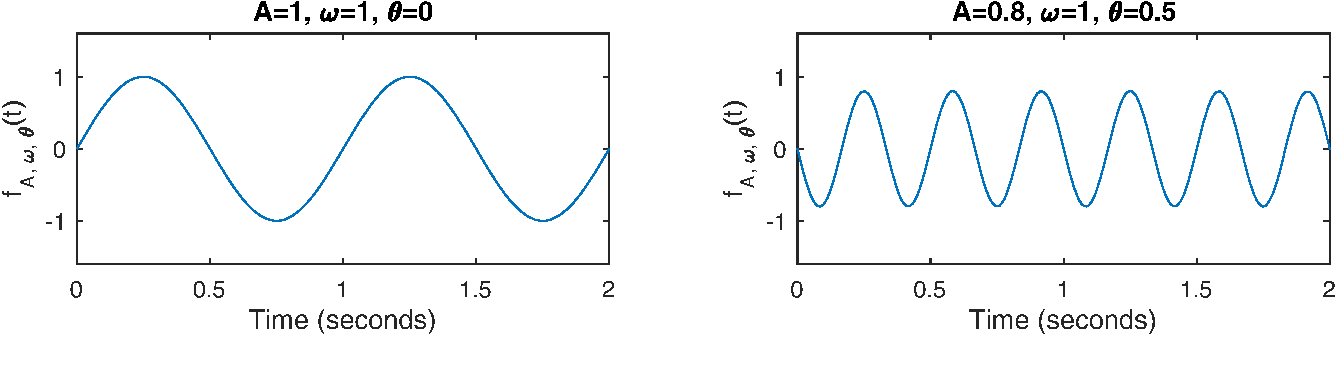
\includegraphics[width=12cm]{figures/fig_sines.pdf}
\vspace*{-0cm}
\caption{Sine functions with different amplitudes $A$, frequencies $\omega$ and phases $\theta$ can be
calculated as $f_{A, \omega, \theta}(t) = A \sin(2\pi (\omega t-\theta))$.}
\label{figure:signals}
\end{figure}


%\begin{figure}[t]
%\centering
%\psset{xunit=1cm, yunit=1cm}
%\begin{pspicture}(0,0)(5,2) % (coordinate system origin)(width and height in centimeters)
%    \psgrid
%\end{pspicture}
%\caption{A simple grid sometimes helps to find the right coordinates in the figure.}
%\label{figure:grid}
%\end{figure}


\begin{figure}[t]
\centering

\includegraphics[width=4cm]{figures/Smiley.pdf}
\vspace*{-0cm}
\caption{Pixel graphics can also be included, but in low resolution it looks terrible and in high resolution is takes ages to load.}
\label{figure:smiley}
\end{figure}



%%%%%%%%%%%%%%%%%%%%%%%%%%%%%%%%%%%%%%%%%%%%%%%%%%%%%%%%%%%%%%%%%%%%%%%%%%%%%%%%%%%%%%%
\section{Theorem-like Constructs}
\label{section:constructs}
%%%%%%%%%%%%%%%%%%%%%%%%%%%%%%%%%%%%%%%%%%%%%%%%%%%%%%%%%%%%%%%%%%%%%%%%%%%%%%%%%%%%%%%
Other common constructs that may occur in your thesis are
the forms for logical constructs like theorems, axioms,
corollaries and proofs. See the following example:

\begin{Theorem}
Let $f$ be continuous on $[a,b]$.  If $G$ is
an antiderivative for $f$ on $[a,b]$, then
\begin{align}
  \int^{b}_{a}f(t)dt = G(b) - G(a).
\end{align}
\end{Theorem}

The following is a definition:
\begin{Definition}
If $z$ is irrational, then by $e^z$ we mean the
unique number which has logarithm $z$:
\begin{align}
  \log e^z = z.
\end{align}
\end{Definition}

%%%%%%%%%%%%%%%%%%%%%%%%%%%%%%%%%%%%%%%%%%%%%%%%%%%%%%%%%%%%%%%%%%%%%%%%%%%%%%%%%%%%%%%
\chapter{Conclusions}
\label{chapter:conclusions}
%%%%%%%%%%%%%%%%%%%%%%%%%%%%%%%%%%%%%%%%%%%%%%%%%%%%%%%%%%%%%%%%%%%%%%%%%%%%%%%%%%%%%%%

Draw the conclusions in the big picture of the thesis! Then, indicate future work.

%%%%%%%%%%%%%%%%%%%%%%%%%%%%%%%%%%%%%%%%%%%%%%%%%%%%%%%%%%%%%%%%%%%%%%%%%%%%%%%%%%%%%%%%%%%%%
% Appendix
%%%%%%%%%%%%%%%%%%%%%%%%%%%%%%%%%%%%%%%%%%%%%%%%%%%%%%%%%%%%%%%%%%%%%%%%%%%%%%%%%%%%%%%%%%%%%
\cleardoublepage{}
\appendix
%%%%%%%%%%%%%%%%%%%%%%%%%%%%%%%%%%%%%%%%%%%%%%%%%%%%%%%%%%%%%%%%%%%%%%%%%%%%%%%%%%%%%%%
\chapter{Source Code}
\label{chapter:source_code}
%%%%%%%%%%%%%%%%%%%%%%%%%%%%%%%%%%%%%%%%%%%%%%%%%%%%%%%%%%%%%%%%%%%%%%%%%%%%%%%%%%%%%%%

In this chapter, the headers of selected \MATLAB{} functions created during the writing of this thesis are reproduced. The headers contain information about the name of the described function and its input/output behavior.

\section*{Feature Extraction}
The \texttt{file\_to\_feature} function is used as a wrapper for several low-level functions that perform feature extraction or loading of precomputed features.

Sample usage:\\
\scriptsize
\verb|[f_pitch, f_peaks] = file_to_feature('features', 'pathetique.wav');|

\begin{verbatim}
%%%%%%%%%%%%%%%%%%%%%%%%%%%%%%%%%%%%%%%%%%%%%%%%%%%%%%%%%%%%%%%%%%%%%%%%%%%
% Name: file_to_feature
% Version: 1.0
% Date: 11.05.2010
% Programmer: John Q. Public
%
% Description:
%   Load or compute features for audio and MIDI files
%
% Input:
% - dirname: Directory where the file or features are located
% - filename: Name of the file for which to load/compute features
% - parameter
%            .win_len: Window length used for STMSP feature generation
%            .win_res: Window resolution
%
% Output:
% - f_pitch: Pitch features (STMSP)
% - f_peaks: Energy peaks for onset computation
% - f_onsets: Precise onsets (only generated in case of MIDI input data)
%%%%%%%%%%%%%%%%%%%%%%%%%%%%%%%%%%%%%%%%%%%%%%%%%%%%%%%%%%%%%%%%%%%%%%%%%%%
\end{verbatim}
\normalsize

%%%%%%%%%%%%%%%%%%%%%%%%%%%%%%%%%%%%%%%%%%%%%%%%%%%%%%%%%%%%%%%%%%%%%%%%%%%%%%%%%%%%%%%%%%%%
% Bibliography
%%%%%%%%%%%%%%%%%%%%%%%%%%%%%%%%%%%%%%%%%%%%%%%%%%%%%%%%%%%%%%%%%%%%%%%%%%%%%%%%%%%%%%%%%%%%
\cleardoublepage{}
{
\small
\addcontentsline{toc}{chapter}{Bibliography}
\bibliographystyle{siam}
\bibliography{bibliography}
}
\cleardoublepage{}


\end{document}
